% Options for packages loaded elsewhere
\PassOptionsToPackage{unicode}{hyperref}
\PassOptionsToPackage{hyphens}{url}
\PassOptionsToPackage{dvipsnames,svgnames,x11names}{xcolor}
%
\documentclass[
  xelatex,
  ja=standard]{bxjsarticle}

\usepackage{amsmath,amssymb}
\usepackage{iftex}
\ifPDFTeX
  \usepackage[T1]{fontenc}
  \usepackage[utf8]{inputenc}
  \usepackage{textcomp} % provide euro and other symbols
\else % if luatex or xetex
  \usepackage{unicode-math}
  \defaultfontfeatures{Scale=MatchLowercase}
  \defaultfontfeatures[\rmfamily]{Ligatures=TeX,Scale=1}
\fi
\usepackage{lmodern}
\ifPDFTeX\else  
    % xetex/luatex font selection
  \setmainfont[BoldFont=Noto Sans CJK JP]{Noto Serif CJK JP}
\fi
% Use upquote if available, for straight quotes in verbatim environments
\IfFileExists{upquote.sty}{\usepackage{upquote}}{}
\IfFileExists{microtype.sty}{% use microtype if available
  \usepackage[]{microtype}
  \UseMicrotypeSet[protrusion]{basicmath} % disable protrusion for tt fonts
}{}
\makeatletter
\@ifundefined{KOMAClassName}{% if non-KOMA class
  \IfFileExists{parskip.sty}{%
    \usepackage{parskip}
  }{% else
    \setlength{\parindent}{0pt}
    \setlength{\parskip}{6pt plus 2pt minus 1pt}}
}{% if KOMA class
  \KOMAoptions{parskip=half}}
\makeatother
\usepackage{xcolor}
\setlength{\emergencystretch}{3em} % prevent overfull lines
\setcounter{secnumdepth}{5}
% Make \paragraph and \subparagraph free-standing
\ifx\paragraph\undefined\else
  \let\oldparagraph\paragraph
  \renewcommand{\paragraph}[1]{\oldparagraph{#1}\mbox{}}
\fi
\ifx\subparagraph\undefined\else
  \let\oldsubparagraph\subparagraph
  \renewcommand{\subparagraph}[1]{\oldsubparagraph{#1}\mbox{}}
\fi


\providecommand{\tightlist}{%
  \setlength{\itemsep}{0pt}\setlength{\parskip}{0pt}}\usepackage{longtable,booktabs,array}
\usepackage{calc} % for calculating minipage widths
% Correct order of tables after \paragraph or \subparagraph
\usepackage{etoolbox}
\makeatletter
\patchcmd\longtable{\par}{\if@noskipsec\mbox{}\fi\par}{}{}
\makeatother
% Allow footnotes in longtable head/foot
\IfFileExists{footnotehyper.sty}{\usepackage{footnotehyper}}{\usepackage{footnote}}
\makesavenoteenv{longtable}
\usepackage{graphicx}
\makeatletter
\def\maxwidth{\ifdim\Gin@nat@width>\linewidth\linewidth\else\Gin@nat@width\fi}
\def\maxheight{\ifdim\Gin@nat@height>\textheight\textheight\else\Gin@nat@height\fi}
\makeatother
% Scale images if necessary, so that they will not overflow the page
% margins by default, and it is still possible to overwrite the defaults
% using explicit options in \includegraphics[width, height, ...]{}
\setkeys{Gin}{width=\maxwidth,height=\maxheight,keepaspectratio}
% Set default figure placement to htbp
\makeatletter
\def\fps@figure{htbp}
\makeatother

\renewcommand{\thefootnote}{\arabic{footnote}}
\makeatletter
\@ifpackageloaded{tcolorbox}{}{\usepackage[skins,breakable]{tcolorbox}}
\@ifpackageloaded{fontawesome5}{}{\usepackage{fontawesome5}}
\definecolor{quarto-callout-color}{HTML}{909090}
\definecolor{quarto-callout-note-color}{HTML}{0758E5}
\definecolor{quarto-callout-important-color}{HTML}{CC1914}
\definecolor{quarto-callout-warning-color}{HTML}{EB9113}
\definecolor{quarto-callout-tip-color}{HTML}{00A047}
\definecolor{quarto-callout-caution-color}{HTML}{FC5300}
\definecolor{quarto-callout-color-frame}{HTML}{acacac}
\definecolor{quarto-callout-note-color-frame}{HTML}{4582ec}
\definecolor{quarto-callout-important-color-frame}{HTML}{d9534f}
\definecolor{quarto-callout-warning-color-frame}{HTML}{f0ad4e}
\definecolor{quarto-callout-tip-color-frame}{HTML}{02b875}
\definecolor{quarto-callout-caution-color-frame}{HTML}{fd7e14}
\makeatother
\makeatletter
\makeatother
\makeatletter
\makeatother
\makeatletter
\@ifpackageloaded{caption}{}{\usepackage{caption}}
\AtBeginDocument{%
\ifdefined\contentsname
  \renewcommand*\contentsname{目次}
\else
  \newcommand\contentsname{目次}
\fi
\ifdefined\listfigurename
  \renewcommand*\listfigurename{図一覧}
\else
  \newcommand\listfigurename{図一覧}
\fi
\ifdefined\listtablename
  \renewcommand*\listtablename{表一覧}
\else
  \newcommand\listtablename{表一覧}
\fi
\ifdefined\figurename
  \renewcommand*\figurename{図}
\else
  \newcommand\figurename{図}
\fi
\ifdefined\tablename
  \renewcommand*\tablename{表}
\else
  \newcommand\tablename{表}
\fi
}
\@ifpackageloaded{float}{}{\usepackage{float}}
\floatstyle{ruled}
\@ifundefined{c@chapter}{\newfloat{codelisting}{h}{lop}}{\newfloat{codelisting}{h}{lop}[chapter]}
\floatname{codelisting}{コード}
\newcommand*\listoflistings{\listof{codelisting}{コード一覧}}
\makeatother
\makeatletter
\@ifpackageloaded{caption}{}{\usepackage{caption}}
\@ifpackageloaded{subcaption}{}{\usepackage{subcaption}}
\makeatother
\makeatletter
\@ifpackageloaded{tcolorbox}{}{\usepackage[skins,breakable]{tcolorbox}}
\makeatother
\makeatletter
\@ifundefined{shadecolor}{\definecolor{shadecolor}{rgb}{.97, .97, .97}}
\makeatother
\makeatletter
\makeatother
\makeatletter
\makeatother
\ifLuaTeX
\usepackage[bidi=basic]{babel}
\else
\usepackage[bidi=default]{babel}
\fi
\babelprovide[main,import]{japanese}
% get rid of language-specific shorthands (see #6817):
\let\LanguageShortHands\languageshorthands
\def\languageshorthands#1{}
\ifLuaTeX
  \usepackage{selnolig}  % disable illegal ligatures
\fi
\usepackage[]{natbib}
\bibliographystyle{jecon}
\IfFileExists{bookmark.sty}{\usepackage{bookmark}}{\usepackage{hyperref}}
\IfFileExists{xurl.sty}{\usepackage{xurl}}{} % add URL line breaks if available
\urlstyle{same} % disable monospaced font for URLs
\hypersetup{
  pdftitle={戦争と外交},
  pdfauthor={土井翔平},
  pdflang={ja},
  colorlinks=true,
  linkcolor={NavyBlue},
  filecolor={Maroon},
  citecolor={NavyBlue},
  urlcolor={NavyBlue},
  pdfcreator={LaTeX via pandoc}}

\title{戦争と外交}
\usepackage{etoolbox}
\makeatletter
\providecommand{\subtitle}[1]{% add subtitle to \maketitle
  \apptocmd{\@title}{\par {\large #1 \par}}{}{}
}
\makeatother
\subtitle{国際公共政策学}
\author{土井翔平}
\date{2023-04-25}

\begin{document}
\maketitle
\ifdefined\Shaded\renewenvironment{Shaded}{\begin{tcolorbox}[boxrule=0pt, frame hidden, breakable, enhanced, borderline west={3pt}{0pt}{shadecolor}, sharp corners, interior hidden]}{\end{tcolorbox}}\fi

\hypertarget{ux306fux3058ux3081ux306b}{%
\section*{はじめに}\label{ux306fux3058ux3081ux306b}}
\addcontentsline{toc}{section}{はじめに}

なぜ戦争は(社会的に望ましくないのに)起こるのか?

\begin{enumerate}
\def\labelenumi{\arabic{enumi}.}
\tightlist
\item
  \textbf{⼈間}は本能的に争うから。戦争を好きな⼈間が政治的指導者になるから。

  \begin{itemize}
  \tightlist
  \item
    確かに、(少なくとも一部の)人間は好戦的な性格を持ち、戦争を行うこと自体が目的である場合もある。
  \item
    戦争が起こった場合=当事者の政治家や⺠族が戦争好きだった(循環論法)
  \item
    安全保障政策\(\leadsto\)好戦的な人間を排除、性格を変える(生産的?)
  \end{itemize}
\item
  \textbf{アナーキー}な国際社会では戦争をしても罰せられないから。戦争を防ぐアクターがいないから。

  \begin{itemize}
  \tightlist
  \item
    確かに、警察や司法のように違法行為を取り締まって、処罰する存在はいない。
  \item
    犯罪も全て抑止されていない。主権国家内でも内戦は起こる。
  \item
    安全保障政策\(\leadsto\)アナーキーな国際社会を変えて、世界規模の中央集権的政治体制を構築する(現実的?)
  \end{itemize}
\end{enumerate}

いずれにせよ、人間の本性や国際社会の構造だけでは、特定の時代や地域で戦争や暴力が多いことを説明できない。

\(\leadsto\)なぜ戦争が、どのような状況で\textbf{選択}されるのか?

\begin{itemize}
\tightlist
\item
  戦争は自然災害のようにある日、突然起こるものではない。
\end{itemize}

\hypertarget{ux8ab2ux984cux6587ux732e}{%
\subsection*{課題文献}\label{ux8ab2ux984cux6587ux732e}}
\addcontentsline{toc}{subsection}{課題文献}

\begin{itemize}
\tightlist
\item
  強制外交と安心供与

  \begin{itemize}
  \tightlist
  \item
    \citet[第3章]{nakanishi2013}
  \end{itemize}
\item
  戦争の交渉モデル

  \begin{itemize}
  \tightlist
  \item
    \citet[第2章]{tago2020}
  \item
    \citet[第10章]{sunahara2020}
  \item
    \citet[第2章]{sakamoto2020}
  \item
    \citet[第4章]{ohshiba2018}
  \item
    \citet[第11章]{asako2018}
  \item
    \citet[第6章]{okada2020}
  \item
    \citet[第1章]{ishiguro2019}
  \end{itemize}
\end{itemize}

\hypertarget{ux6226ux4e89ux306eux69cbux9020}{%
\section{戦争の構造}\label{ux6226ux4e89ux306eux69cbux9020}}

あらゆる戦争は、様々な面で\textbf{異なっている}。

\begin{itemize}
\tightlist
\item
  当事国の政策決定者(政治家)、歴史、政治経済状況、国際環境
\end{itemize}

しかし、異なる点を強調しすぎるとある戦争に関する情報は他の戦争について役に立たない。

\(\leadsto\)様々な戦争に共通する構造、要因に着目

\hypertarget{ux653fux6cbbux306eux624bux6bb5ux3068ux3057ux3066ux306eux6226ux4e89}{%
\subsection{政治の手段としての戦争}\label{ux653fux6cbbux306eux624bux6bb5ux3068ux3057ux3066ux306eux6226ux4e89}}

カール・フォン・クラウゼヴィッツ(「戦争論」)の戦争の定義\citep{clausewitz2020}

\begin{quote}
戦争とは他の⼿段をもってする政治の継続である。
\end{quote}

\begin{quote}
戦争とは、敵を強制してわれわれの意志を遂⾏させるために⽤いられる暴⼒⾏為である。
\end{quote}

\begin{figure}[htpb]

{\centering \includegraphics[width=0.5\textwidth,height=\textheight]{war_and_diplomacy_files/mediabag/Carl_von_Clausewitz.PNG}

}

\caption{\href{https://commons.wikimedia.org/wiki/File:Carl_von_Clausewitz.PNG}{カール・フォン・クラウゼヴィッツ}}

\end{figure}

戦争:政治的目的を実現する\textbf{手段}、政治(外交)の延長線上

\begin{itemize}
\tightlist
\item
  戦争それ自体が\textbf{目的}ではない(そうあるべきではない)。
\item
  戦争\textbf{以外}の手段でも政治的目的は達成しうる。
\end{itemize}

\(\leadsto\)「なぜ戦争が起こるのか」=「なぜ外交が失敗したのか」\citep{fearon1995}

\hypertarget{ux653fux6cbbux304cux767bux5834ux3059ux308bux3068ux304d}{%
\subsection{政治が登場するとき}\label{ux653fux6cbbux304cux767bux5834ux3059ux308bux3068ux304d}}

「政治とはなにか」は難しい問い\(\leadsto\)どのようなときに政治が登場するかを考える。

\hypertarget{ux8907ux6570ux306eux30a2ux30afux30bfux30fc}{%
\subsubsection{複数のアクター}\label{ux8907ux6570ux306eux30a2ux30afux30bfux30fc}}

一人で意思決定できる場合は政治は登場しない。

\begin{itemize}
\tightlist
\item
  例、一人で夕飯になにを食べるか
\end{itemize}

\(\leadsto\)複数の人の間で意思決定を行う時に政治が登場する。

\textbf{アクター}
(actor):自律的に(他者から影響を受けつつも)意思決定を行う存在

\begin{itemize}
\tightlist
\item
  国際社会では主権国家が主たるアクター
\item
  国家を動かす政治家、官僚、企業、市民
\item
  国境を越えて活動する国際機関、NGO、テロリスト
\end{itemize}

\hypertarget{ux5229ux5bb3ux306eux5bfeux7acb}{%
\subsubsection{利害の対立}\label{ux5229ux5bb3ux306eux5bfeux7acb}}

全てのアクターが同じ目的、利害関心を持っている場合も政治は登場しない。

\begin{itemize}
\tightlist
\item
  例、GWに授業をするか
\end{itemize}

\(\leadsto\)利害が対立する時に政治が登場する。

\textbf{利益} (interest):アクターが追求するもの

\begin{itemize}
\tightlist
\item
  経済的利益、自己利益に限定されない。
\end{itemize}

\textbf{国益} (national interest):国家が追求する利益

\begin{enumerate}
\def\labelenumi{\arabic{enumi}.}
\tightlist
\item
  最も基本的な国益は\textbf{安全保障} (security)

  \begin{itemize}
  \tightlist
  \item
    \textbf{生存} (survival)
    を維持できていれば十分〜自国の独立への脅威が小さい
  \end{itemize}
\item
  安全保障を達成するための\textbf{権力} (power) や\textbf{国力}
  (national capability)\footnote{国力と安全保障は密接に関係しているが、必ずしも等しいものではない。}

  \begin{itemize}
  \tightlist
  \item
    相手に意に反する行動を取らせることができる能力という関係性に基づく見方
  \item
    軍事力や経済力など権力行使の資源に着目する見方
  \item
    いずれにせよ、国力とは\textbf{関係のある他の国の国力との比較において決まる}と考えられる。
  \end{itemize}
\item
  経済的な\textbf{富} (wealth)

  \begin{itemize}
  \tightlist
  \item
    住民の生活水準や福祉 (well-being)
    の向上\(\leadsto\)しばしば為政者の権力維持
  \item
    経済力や技術力を用いて軍事力に投資\(\leadsto\)国力の向上

    \begin{itemize}
    \tightlist
    \item
      軍事力のために経済的富を放棄しなければいけないという\textbf{トレードオフ}
    \end{itemize}
  \end{itemize}
\item
  \textbf{領土} (territory)

  \begin{itemize}
  \tightlist
  \item
    軍事力や経済力の源泉
  \item
    有限かつ交換不可能である点で特殊
  \item
    産業革命以前:領土の広さ=生産力や市場の規模=国力資\(\leadsto\)領土紛争\footnote{この時期は経済力の伸長のために領土の拡大を行い、統治のために過剰な軍事力が必要になった結果、帝国が没落していったという見方もある\citep{kennedy1993}。}
  \item
    産業革命やフランス革命以降:領土を巡る争いに2つの相反する効果

    \begin{enumerate}
    \def\labelenumii{\arabic{enumii}.}
    \tightlist
    \item
      領土の経済的価値は低下&ナショナリズムの興隆により統治費用が拡大\(\leadsto\)領土を拡大する利益の減少
    \item
      ナショナリズム\(\leadsto\)領土を巡る譲歩の費用も拡大\(\leadsto\)妥協しにくい
    \end{enumerate}
  \end{itemize}
\item
  \textbf{観念}的 (ideational) 要素

  \begin{itemize}
  \tightlist
  \item
    イデオロギーや政治体制、価値観、宗教、評判や名誉
  \item
    実際には、そこから生まれる権力や富?
  \end{itemize}
\end{enumerate}

現代の武力紛争は領土や政策(政府や政治体制を含む)を巡るものが多い。

\hypertarget{ux6226ux4e89ux3068ux5916ux4ea4}{%
\subsection{戦争と外交}\label{ux6226ux4e89ux3068ux5916ux4ea4}}

政治は複数の利害が対立するアクター(国家)の間で展開される。

利害の対立\(\neq\)戦争\(\leadsto\)戦争ではなく外交によって利害対立を解決する。

外交では、国家同士で価値のあるもの、\textbf{財} (goods)
をどのように分割するかについて決定する。

\begin{itemize}
\tightlist
\item
  例、争っている領土をどのように分割するか、どのような政治体制・政策にするか
\item
  \textbf{現状変更}勢力 (revisionist power)/\textbf{現状維持}勢力
  (status quo power)
\end{itemize}

最も単純な交渉は、一方が財を要求するかどうかを決定し、他方が譲歩するかどうかを決定するものである。

\begin{itemize}
\tightlist
\item
  まずはシンプルに2つの国(アクター)が領土を巡って争っている(利害対立)状況を考える。
\end{itemize}

\hypertarget{ux6291ux6b62}{%
\section{抑止}\label{ux6291ux6b62}}

\hypertarget{ux4e00ux822cux6291ux6b62ux3068ux7dcaux6025ux6291ux6b62}{%
\subsection{一般抑止と緊急抑止}\label{ux4e00ux822cux6291ux6b62ux3068ux7dcaux6025ux6291ux6b62}}

\textbf{抑止} (deterrence)
:実行したいこと(つまり戦争)を自制させること

\begin{itemize}
\tightlist
\item
  \textbf{一般抑止}:対立関係にはあるが武力行使や威嚇が顕在化することを防ぐ。\footnote{同盟国への攻撃の抑止を拡大抑止と呼ぶが、それに対して自国への攻撃の抑止を一般(通常)抑止と呼ぶこともある。}
\item
  \textbf{緊急抑止}:現状変更が求められた国際危機において、武力による威嚇で武力行使を防ぐ。
\end{itemize}

\begin{figure}[htpb]

{\centering 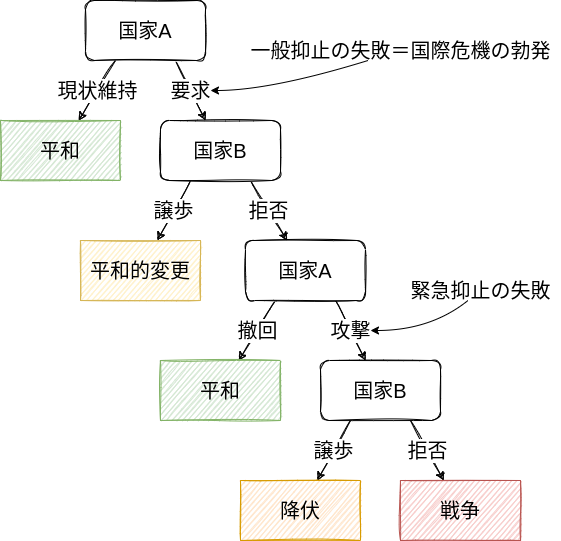
\includegraphics[width=0.8\textwidth,height=\textheight]{figures/crisis.drawio.png}

}

\caption{危機交渉モデル}

\end{figure}

(\textbf{強要} (compellence) :実行したくないことを実行させること)

\textbf{強制外交} (coersion diplomacy):武力や威嚇による抑止や強要

\(\leadsto\)どのような場合に緊急抑止が成功するのか?

\hypertarget{ux30b7ux30caux30eaux30aa1ux7dcaux6025ux6291ux6b62ux306eux7834ux7dbbux6226ux4e89ux306eux56deux907f}{%
\subsection{シナリオ1:緊急抑止の破綻・戦争の回避}\label{ux30b7ux30caux30eaux30aa1ux7dcaux6025ux6291ux6b62ux306eux7834ux7dbbux6226ux4e89ux306eux56deux907f}}

次のような架空の状況を考えてみる。

\begin{tcolorbox}[enhanced jigsaw, titlerule=0mm, rightrule=.15mm, left=2mm, arc=.35mm, toptitle=1mm, toprule=.15mm, opacityback=0, leftrule=.75mm, coltitle=black, colback=white, title=\textcolor{quarto-callout-tip-color}{\faLightbulb}\hspace{0.5em}{国際危機のシナリオ1}, breakable, opacitybacktitle=0.6, bottomrule=.15mm, colbacktitle=quarto-callout-tip-color!10!white, colframe=quarto-callout-tip-color-frame, bottomtitle=1mm]

\begin{itemize}
\tightlist
\item
  国家AとBはとある領土の所有権を巡って争っている。
\item
  国家Aはその領土の20\%を、国家Bは80\%を占領している。
\item
  国家Aはさらにその領土の60\%(つまり、全体で80\%)の割譲をBに求めている。
\item
  仮に戦争が起こった場合、勝利した国が領土を全て占領できる。
\item
  国家Aは50\%の確率で戦争に勝つ見込みである(したがって、国家Bも同様である)。
\item
  しかし、戦争には費用がかかり、それを土地の価値に揃えるとAとBにとって40\%分の価値であるとする。
\end{itemize}

\end{tcolorbox}

仮に戦争が起こった場合、国家AとBは

\[
\textrm{勝利したときの領土} \times \textrm{勝利する確率} - \textrm{戦争の費用} = 1 \times 0.5 - 0.4 = 0.1
\]

の利益を得る。

\begin{figure}[htpb]

{\centering 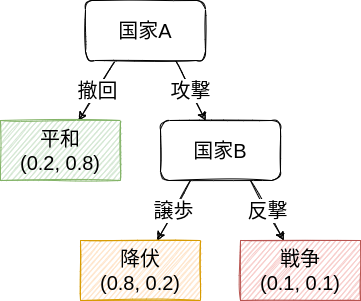
\includegraphics{figures/deterrence1.drawio.png}

}

\caption{危機交渉モデル(シナリオ1)}

\end{figure}

\(\leadsto\)緊急抑止は失敗するが、戦争が起こらない。

\hypertarget{ux30b7ux30caux30eaux30aa2ux7dcaux6025ux6291ux6b62ux306eux6210ux529f}{%
\subsection{シナリオ2:緊急抑止の成功}\label{ux30b7ux30caux30eaux30aa2ux7dcaux6025ux6291ux6b62ux306eux6210ux529f}}

\begin{tcolorbox}[enhanced jigsaw, titlerule=0mm, rightrule=.15mm, left=2mm, arc=.35mm, toptitle=1mm, toprule=.15mm, opacityback=0, leftrule=.75mm, coltitle=black, colback=white, title=\textcolor{quarto-callout-tip-color}{\faLightbulb}\hspace{0.5em}{国際危機のシナリオ2}, breakable, opacitybacktitle=0.6, bottomrule=.15mm, colbacktitle=quarto-callout-tip-color!10!white, colframe=quarto-callout-tip-color-frame, bottomtitle=1mm]

\begin{itemize}
\tightlist
\item
  国家AとBはとある領土の所有権を巡って争っている。
\item
  国家Aはその領土の20\%を、国家Bは80\%を占領している。
\item
  国家Aはさらにその領土の60\%(つまり、全体で80\%)の割譲をBに求めている。
\item
  仮に戦争が起こった場合、勝利した国が領土を全て占領できる。
\item
  国家Aは50\%の確率で戦争に勝つ見込みである(したがって、国家Bも同様である)。
\item
  しかし、戦争には費用がかかり、それを土地の価値に揃えるとAにとって40\%分の、Bにとって20\%分の価値であるとする。
\end{itemize}

\end{tcolorbox}

仮に戦争が起こった場合、国家Bは

\[
\textrm{勝利したときの領土} \times \textrm{勝利する確率} - \textrm{戦争の費用} = 1 \times 0.5 - 0.2 = 0.3
\]

の利益を得る(国家Aはシナリオ1と変わらず)。

\begin{figure}[htpb]

{\centering 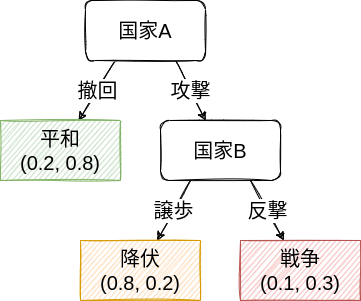
\includegraphics{figures/deterrence2.drawio.png}

}

\caption{危機交渉モデル(シナリオ2)}

\end{figure}

\(\leadsto\)緊急抑止が成功する。

\hypertarget{ux30b7ux30caux30eaux30aa3ux7dcaux6025ux6291ux6b62ux306eux5931ux6557ux6226ux4e89ux306eux52c3ux767a}{%
\subsection{シナリオ3:緊急抑止の失敗・戦争の勃発}\label{ux30b7ux30caux30eaux30aa3ux7dcaux6025ux6291ux6b62ux306eux5931ux6557ux6226ux4e89ux306eux52c3ux767a}}

\begin{tcolorbox}[enhanced jigsaw, titlerule=0mm, rightrule=.15mm, left=2mm, arc=.35mm, toptitle=1mm, toprule=.15mm, opacityback=0, leftrule=.75mm, coltitle=black, colback=white, title=\textcolor{quarto-callout-tip-color}{\faLightbulb}\hspace{0.5em}{国際危機のシナリオ3}, breakable, opacitybacktitle=0.6, bottomrule=.15mm, colbacktitle=quarto-callout-tip-color!10!white, colframe=quarto-callout-tip-color-frame, bottomtitle=1mm]

\begin{itemize}
\tightlist
\item
  国家AとBはとある領土の所有権を巡って争っている。
\item
  国家Aはその領土の20\%を、国家Bは80\%を占領している。
\item
  国家Aはさらにその領土の60\%(つまり、全体で80\%)の割譲をBに求めている。
\item
  仮に戦争が起こった場合、勝利した国が領土を全て占領できる。
\item
  国家Aは50\%の確率で戦争に勝つ見込みである(したがって、国家Bも同様である)。
\item
  しかし、戦争には費用がかかり、それを土地の価値に揃えるとAとBにとって20\%分の価値であるとする。
\end{itemize}

\end{tcolorbox}

仮に戦争が起こった場合、国家AとBは

\[
\textrm{勝利したときの領土} \times \textrm{勝利する確率} - \textrm{戦争の費用} = 1 \times 0.5 - 0.2 = 0.3
\]

の利益を得る。

\begin{figure}[htpb]

{\centering 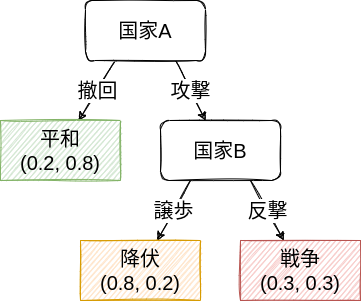
\includegraphics{figures/deterrence3.drawio.png}

}

\caption{危機交渉モデル(シナリオ3)}

\end{figure}

\(\leadsto\)緊急抑止は失敗し、戦争が起こる。

\hypertarget{ux6291ux6b62ux306eux6210ux529f}{%
\subsection{抑止の成功}\label{ux6291ux6b62ux306eux6210ux529f}}

抑止を成功させる条件=(1)国家Bは攻撃をされたら反撃をする&(2)国家Aは攻撃をしない

なぜ、国家Bは反撃を選択したのか?

\begin{itemize}
\tightlist
\item
  戦争から得られる利益>降伏から得られる利益
\end{itemize}

\(\leadsto\)\textbf{現状維持の意図}が大きい。

\[
\begin{split}
&\textrm{戦争の利益} \\
&= \textrm{勝利したときの財} \times \textrm{勝利確}率 - \textrm{戦争費用} \\
&> \textrm{降伏の利益}
\end{split}
\]

現状維持勢力にとって

\begin{itemize}
\tightlist
\item
  争いの対象となっている財の価値が高い
\item
  戦争で勝利する確率が高い
\item
  戦争の費用が小さい
\end{itemize}

ときに反撃しやすい。

なぜ、国家Aは撤回を選択したのか?

\begin{itemize}
\tightlist
\item
  平和から得られる利益>戦争から得られる利益
\end{itemize}

\(\leadsto\)\textbf{現状変更の意図}が小さい。

\[
\begin{split}
&\textrm{戦争の利益} \\
&= \textrm{勝利したときの財} \times \textrm{勝利確}率 - \textrm{戦争費用} \\
&< \textrm{平和の利益}
\end{split}
\]

国家Bは

\begin{itemize}
\tightlist
\item
  \textbf{拒否的抑止}:相手国の勝利する確率を低下させる
\item
  \textbf{懲罰的抑止}:相手国の戦争費用を増加させる
\end{itemize}

によって国家Aを抑止することができる。

\hypertarget{ux4ea4ux6e09}{%
\section{交渉}\label{ux4ea4ux6e09}}

実際には武力行使の前に、\textbf{どのように財を分け合うのか}について交渉はできるはず。

緊急抑止が失敗し、戦争に至るシナリオ3ににおいて、次のような状況を考える。

\begin{tcolorbox}[enhanced jigsaw, titlerule=0mm, rightrule=.15mm, left=2mm, arc=.35mm, toptitle=1mm, toprule=.15mm, opacityback=0, leftrule=.75mm, coltitle=black, colback=white, title=\textcolor{quarto-callout-tip-color}{\faLightbulb}\hspace{0.5em}{国際危機のシナリオ3'}, breakable, opacitybacktitle=0.6, bottomrule=.15mm, colbacktitle=quarto-callout-tip-color!10!white, colframe=quarto-callout-tip-color-frame, bottomtitle=1mm]

\begin{itemize}
\tightlist
\item
  国家Aが領土を半分ずつ国家Bと分け合う提案をする。
\end{itemize}

\end{tcolorbox}

\begin{figure}[htpb]

{\centering 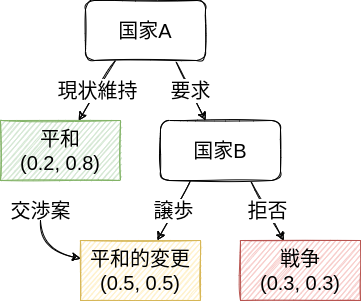
\includegraphics{figures/crisis_bargaining.drawio.png}

}

\caption{危機交渉モデル(シナリオ3')}

\end{figure}

\(\leadsto\)国家AとBは平和的な変更に合意する。

\begin{itemize}
\tightlist
\item
  国家A:戦争よりも分割のほうが望ましい。
\item
  国家B:現状よりも分割は望ましくないが、戦争よりは望ましい。
\end{itemize}

戦争に費用がかかる限り、互いに戦争よりも望ましい財の配分案は\textbf{必ず存在する}\citep{fearon1995}。

\begin{figure}[htpb]

{\centering \includegraphics{war_and_diplomacy_files/mediabag/division_of_korea.png}

}

\caption{\href{https://wonderingmaps.com/korea-division/}{朝鮮戦争}}

\end{figure}

\[
\begin{split}
&\textrm{Aの交渉の利益} + \textrm{Bの交渉の利益} = 0.5 + 0.5 \\
&> 0.3 + 0.3 = \textrm{Aの戦争の利益} + \textrm{Bの戦争の利益}
\end{split}
\]

\hypertarget{ux5b89ux5fc3ux4f9bux4e0e}{%
\section{安心供与}\label{ux5b89ux5fc3ux4f9bux4e0e}}

交渉によって平和的に解決した後に、蒸し返しが起こるかもしれない。

\begin{tcolorbox}[enhanced jigsaw, titlerule=0mm, rightrule=.15mm, left=2mm, arc=.35mm, toptitle=1mm, toprule=.15mm, opacityback=0, leftrule=.75mm, coltitle=black, colback=white, title=\textcolor{quarto-callout-tip-color}{\faLightbulb}\hspace{0.5em}{国際危機のシナリオ4}, breakable, opacitybacktitle=0.6, bottomrule=.15mm, colbacktitle=quarto-callout-tip-color!10!white, colframe=quarto-callout-tip-color-frame, bottomtitle=1mm]

\begin{itemize}
\tightlist
\item
  国家Aが領土を半分ずつ国家Bと分け合う提案をして、Bはこれを受諾した。
\item
  国家Aはさらにその領土の30\%(つまり、全体で80\%)の割譲をBに求めている。
\item
  仮に戦争が起こった場合、勝利した国が領土を全て占領できる。
\item
  国家Aは50\%の確率で戦争に勝つ見込みである(したがって、国家Bも同様である)。
\item
  しかし、戦争には費用がかかり、それを土地の価値に揃えるとAとBにとって20\%分の価値であるとする。
\end{itemize}

\end{tcolorbox}

\begin{figure}[htpb]

{\centering 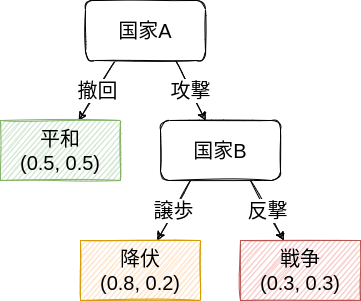
\includegraphics{figures/reassurance1.drawio.png}

}

\caption{危機交渉モデル(シナリオ4)}

\end{figure}

国家Bは武力による威嚇で国家Aの攻撃を抑止

\(\leadsto\)国家Aが平和を選択した後に、国家Bが裏切って攻撃をすることはないだろうか?

\hypertarget{ux56daux4ebaux306eux30b8ux30ecux30f3ux30de}{%
\subsection{囚人のジレンマ}\label{ux56daux4ebaux306eux30b8ux30ecux30f3ux30de}}

\begin{tcolorbox}[enhanced jigsaw, titlerule=0mm, rightrule=.15mm, left=2mm, arc=.35mm, toptitle=1mm, toprule=.15mm, opacityback=0, leftrule=.75mm, coltitle=black, colback=white, title=\textcolor{quarto-callout-tip-color}{\faLightbulb}\hspace{0.5em}{国際危機のシナリオ4'}, breakable, opacitybacktitle=0.6, bottomrule=.15mm, colbacktitle=quarto-callout-tip-color!10!white, colframe=quarto-callout-tip-color-frame, bottomtitle=1mm]

\begin{itemize}
\tightlist
\item
  国家Aが領土を半分ずつ国家Bと分け合う提案をして、Bはこれを受諾した。
\item
  国家Aはさらにその領土の60\%(つまり、全体で80\%)の割譲をBに求めている。
\item
  国家Bはその領土の30\%(つまり、全体で80\%)の返還をBに求めている。
\item
  仮に戦争が起こった場合、勝利した国が領土を全て占領できる。
\item
  国家Aは50\%の確率で戦争に勝つ見込みである(したがって、国家Bも同様である)。
\item
  しかし、戦争には費用がかかり、それを土地の価値に揃えるとAとBにとって20\%分の価値であるとする。
\end{itemize}

\end{tcolorbox}

\begin{figure}[htpb]

{\centering 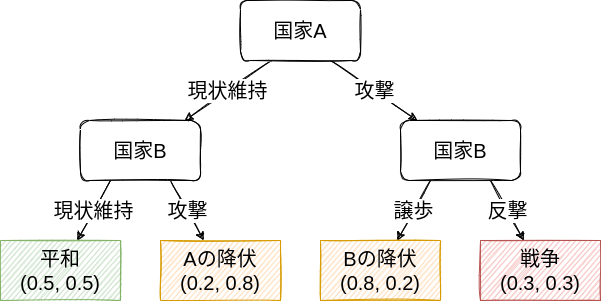
\includegraphics{figures/reassurance2.drawio.png}

}

\caption{危機交渉モデル(シナリオ4')}

\end{figure}

もし国家Bが裏切って攻撃をしてくる場合\(\leadsto\)それを予期した国家Aは戦争を行う。

このような状況を\textbf{囚人のジレンマ} (prisoners' dilemma)
と呼ぶ。\footnote{実際には囚人ではなく容疑者である。}

\begin{tcolorbox}[enhanced jigsaw, titlerule=0mm, rightrule=.15mm, left=2mm, arc=.35mm, toptitle=1mm, toprule=.15mm, opacityback=0, leftrule=.75mm, coltitle=black, colback=white, title=\textcolor{quarto-callout-tip-color}{\faLightbulb}\hspace{0.5em}{囚人のジレンマ}, breakable, opacitybacktitle=0.6, bottomrule=.15mm, colbacktitle=quarto-callout-tip-color!10!white, colframe=quarto-callout-tip-color-frame, bottomtitle=1mm]

\begin{itemize}
\tightlist
\item
  とある事件の容疑者としてAとBが逮捕される。
\item
  しかし、証拠が不十分で、検察は二人を軽微な犯罪でしか起訴できない。
\item
  もし、二人共が黙秘をすれば罰金刑だけが課される。
\item
  しかし、もし自白をすれば罰金刑を免除されるが、相手が自白した場合は証拠となって懲役刑が課せられる。
\end{itemize}

\end{tcolorbox}

\begin{figure}[htpb]

{\centering 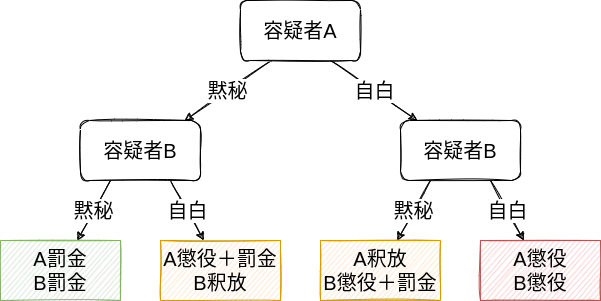
\includegraphics{figures/prisoners_dilemma.drawio.png}

}

\caption{囚人のジレンマ}

\end{figure}

二人は黙秘を続けてるのか、自白するのか?

\(\leadsto\)お互いに黙秘を貫けば罰金で済むのに、互いに自白して懲役刑となる。

\begin{itemize}
\tightlist
\item
  囚人のジレンマは協力問題の典型例\(\leadsto\)安全保障に限らず様々な場面で登場する。
\end{itemize}

国際危機においても、互いに攻撃をしなければ平和だったのに、互いに攻撃を選択して戦争になる。

\hypertarget{ux9e7fux72e9ux308aux30b2ux30fcux30e0}{%
\subsection{鹿狩りゲーム}\label{ux9e7fux72e9ux308aux30b2ux30fcux30e0}}

戦争を回避するには、抑止だけでなく「こちらからは攻撃をしない」という約束、\textbf{安心供与}
(reassurance) も必要になる。

\begin{tcolorbox}[enhanced jigsaw, titlerule=0mm, rightrule=.15mm, left=2mm, arc=.35mm, toptitle=1mm, toprule=.15mm, opacityback=0, leftrule=.75mm, coltitle=black, colback=white, title=\textcolor{quarto-callout-tip-color}{\faLightbulb}\hspace{0.5em}{国際危機のシナリオ4'\,'}, breakable, opacitybacktitle=0.6, bottomrule=.15mm, colbacktitle=quarto-callout-tip-color!10!white, colframe=quarto-callout-tip-color-frame, bottomtitle=1mm]

\begin{itemize}
\tightlist
\item
  もし一方的な武力行使を行った場合、領土の40\%の価値の費用を被る。
\end{itemize}

\end{tcolorbox}

\begin{itemize}
\tightlist
\item
  例、政権維持が困難(落選やクーデタ)、国際社会からの非難や経済制裁
\end{itemize}

\begin{figure}[htpb]

{\centering 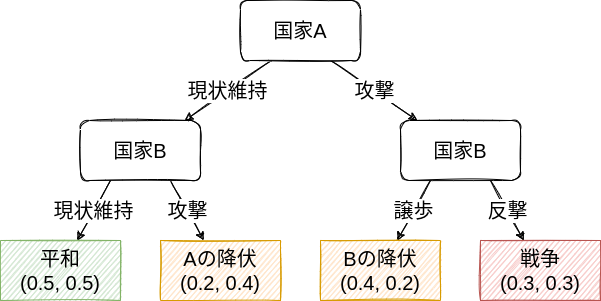
\includegraphics{figures/reassurance3.drawio.png}

}

\caption{危機交渉モデル(シナリオ4')}

\end{figure}

\begin{itemize}
\tightlist
\item
  このような状況は\textbf{鹿狩り} (stag hunt) ゲームと呼ぶ。
\end{itemize}

\(\leadsto\)国家Bは攻撃するよりも平和を求めるので、安心供与に成功する。

\hypertarget{ux6226ux4e89ux306eux539fux56e0}{%
\section{戦争の原因}\label{ux6226ux4e89ux306eux539fux56e0}}

政治が登場するのは、複数の国家の利害が対立しているとき(ことがある)であるが、戦争になるとは限らない。

\(\leadsto\)戦争以外の手段(外交)によって対立を解決することはできる。

\begin{itemize}
\tightlist
\item
  抑止:武力の威嚇によって攻撃を防ぐ。
\item
  交渉:利害を調整して平和的に現状を変更する。
\item
  安心供与:一方的に攻撃をしない約束をする。
\end{itemize}

\(\leadsto\)これらの外交が破綻したときに戦争は生じる(どのようなとき?)。

\hypertarget{ux60c5ux5831ux306eux975eux5bfeux79f0ux6027}{%
\subsection{情報の非対称性}\label{ux60c5ux5831ux306eux975eux5bfeux79f0ux6027}}

これまでの議論は非現実的な箇所がある。

\begin{itemize}
\tightlist
\item
  国家Bが本当に反撃する\textbf{決意} (resolve) があるのか?

  \begin{itemize}
  \tightlist
  \item
    戦争の利益が高い・費用が低い=戦争を行う決意が高い
  \end{itemize}
\item
  \textbf{情報の非対称性} (asymmetric information)
  :一方だけが情報を持っていること
\end{itemize}

\begin{tcolorbox}[enhanced jigsaw, titlerule=0mm, rightrule=.15mm, left=2mm, arc=.35mm, toptitle=1mm, toprule=.15mm, opacityback=0, leftrule=.75mm, coltitle=black, colback=white, title=\textcolor{quarto-callout-tip-color}{\faLightbulb}\hspace{0.5em}{国際危機のシナリオ2'}, breakable, opacitybacktitle=0.6, bottomrule=.15mm, colbacktitle=quarto-callout-tip-color!10!white, colframe=quarto-callout-tip-color-frame, bottomtitle=1mm]

\begin{itemize}
\tightlist
\item
  国家AとBはとある領土の所有権を巡って争っている。
\item
  国家Aはその領土の20\%を、国家Bは80\%を占領している。
\item
  国家Aはさらにその領土の60\%(つまり、全体で80\%)の割譲をBに求めている。
\item
  仮に戦争が起こった場合、勝利した国が領土を全て占領できる。
\item
  国家Aは50\%の確率で戦争に勝つ見込みである(したがって、国家Bも同様である)。
\item
  しかし、戦争には費用がかかり、それを土地の価値に揃えるとAにとって40\%分の価値であるとする。
\item
  ただし、\textbf{国家AにとってBの戦争の費用は分からない}。
\end{itemize}

\end{tcolorbox}

\begin{figure}[htpb]

{\centering 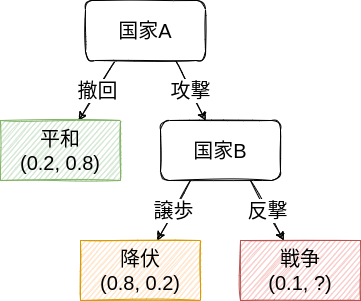
\includegraphics{figures/deterrence_information.drawio.png}

}

\caption{危機交渉モデル(シナリオ2')}

\end{figure}

抑止・交渉の破綻

\begin{itemize}
\tightlist
\item
  国家Aが国家Bの決意が低いと\textbf{誤認} (misperception)
  する=抑止の\textbf{信憑性} (credibility)
  が低い\(\leadsto\)国家Aは国家Bが譲歩するだろうと思って攻撃・過剰な要求
\item
  実際は国家Bは反撃する決意を持っている場合\(\leadsto\)戦争
\end{itemize}

\hypertarget{ux30c1ux30fcux30d7ux30c8ux30fcux30af}{%
\subsubsection{チープ・トーク}\label{ux30c1ux30fcux30d7ux30c8ux30fcux30af}}

\begin{tcolorbox}[enhanced jigsaw, titlerule=0mm, rightrule=.15mm, left=2mm, arc=.35mm, toptitle=1mm, toprule=.15mm, opacityback=0, leftrule=.75mm, coltitle=black, colback=white, title=\textcolor{quarto-callout-tip-color}{\faLightbulb}\hspace{0.5em}{国際危機のシナリオ2'\,'}, breakable, opacitybacktitle=0.6, bottomrule=.15mm, colbacktitle=quarto-callout-tip-color!10!white, colframe=quarto-callout-tip-color-frame, bottomtitle=1mm]

\begin{itemize}
\tightlist
\item
  ただし、国家Bは国家Aに対して「攻撃されたら反撃するぞ」と脅した。
\end{itemize}

\end{tcolorbox}

\begin{figure}[htpb]

{\centering 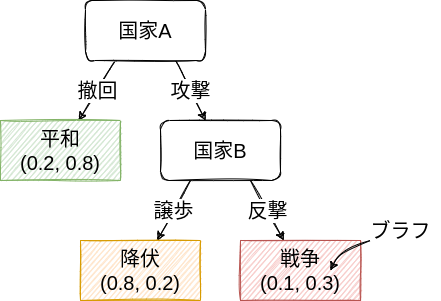
\includegraphics{figures/cheap_talk.drawio.png}

}

\caption{危機交渉モデル(シナリオ2'\,')}

\end{figure}

\begin{itemize}
\tightlist
\item
  こけおどし、\textbf{はったり} (bluff) 、\textbf{チープ・トーク} (cheap
  talk)
  :発信することに費用のかからないメッセージ\(\leadsto\)誰にでも(つまり、決意の低い場合でも)言える。
\item
  「話し合えば分かる」ほど現実は甘くはない。
\end{itemize}

\(\leadsto\)意図を伝達するには費用のかかる行動が必要

\begin{itemize}
\tightlist
\item
  \textbf{コストリー・シグナル} (costly signal) :費用のかかるメッセージ
\end{itemize}

\hypertarget{ux30a2ux30c1ux30bdux30f3ux30e9ux30a4ux30f3}{%
\subsubsection{アチソン・ライン}\label{ux30a2ux30c1ux30bdux30f3ux30e9ux30a4ux30f3}}

1950年にアメリカ国務長官のアチソン:東アジアにおける不後退防衛線(アチソン・ライン)を設定\(\leadsto\)朝鮮半島は範囲外

\begin{figure}[htpb]

{\centering \includegraphics{war_and_diplomacy_files/mediabag/640px-Acheson_line_k.png}

}

\caption{\href{https://commons.wikimedia.org/wiki/File:Acheson_line_ko.svg}{アチソン・ライン}}

\end{figure}

\begin{itemize}
\tightlist
\item
  わざわざアメリカに不利益となるようなシグナル\(\leadsto\)信憑性が高いと判断
\end{itemize}

6月に北朝鮮が韓国に侵攻したため(\textbf{朝鮮戦争})\(\leadsto\)
9月にはアメリカが参戦し、「北進統一」を目指す。

\begin{itemize}
\tightlist
\item
  中国は介入の威嚇を行ったが、韓国・アメリカ軍は北進
\item
  中国の義勇兵が参戦し、戦線を38度線まで押し返す。
\item
  中国の威嚇は決意が低くてもできる点で信憑性が低かったと判断
\end{itemize}

\hypertarget{ux30b3ux30dfux30c3ux30c8ux30e1ux30f3ux30c8ux554fux984c}{%
\subsection{コミットメント問題}\label{ux30b3ux30dfux30c3ux30c8ux30e1ux30f3ux30c8ux554fux984c}}

コミットメント問題:安心供与の約束・\textbf{コミットメント} (commitment)
の信憑性がない\(\leadsto\)戦争

\begin{tcolorbox}[enhanced jigsaw, titlerule=0mm, rightrule=.15mm, left=2mm, arc=.35mm, toptitle=1mm, toprule=.15mm, opacityback=0, leftrule=.75mm, coltitle=black, colback=white, title=\textcolor{quarto-callout-tip-color}{\faLightbulb}\hspace{0.5em}{国際危機のシナリオ4'}, breakable, opacitybacktitle=0.6, bottomrule=.15mm, colbacktitle=quarto-callout-tip-color!10!white, colframe=quarto-callout-tip-color-frame, bottomtitle=1mm]

\begin{itemize}
\tightlist
\item
  国家Aが領土を半分ずつ国家Bと分け合う提案をして、Bはこれを受諾した。
\item
  国家Aはさらにその領土の60\%(つまり、全体で80\%)の割譲をBに求めている。
\item
  国家Bはその領土の30\%(つまり、全体で80\%)の返還をBに求めている。
\item
  仮に戦争が起こった場合、勝利した国が領土を全て占領できる。
\item
  国家Aは50\%の確率で戦争に勝つ見込みである(したがって、国家Bも同様である)。
\item
  しかし、戦争には費用がかかり、それを土地の価値に揃えるとAとBにとって20\%分の価値であるとする。
\end{itemize}

\end{tcolorbox}

\begin{figure}[htpb]

{\centering 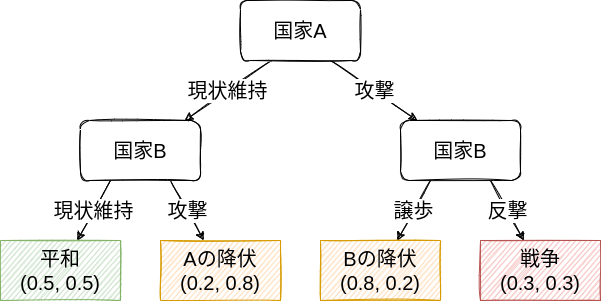
\includegraphics{figures/reassurance2.drawio.png}

}

\caption{危機交渉モデル(シナリオ4')}

\end{figure}

\begin{itemize}
\tightlist
\item
  現時点で平和や交渉による解決を実現しても、将来、攻撃や再交渉をされるかもしれない\(\leadsto\)そうなる前に攻撃
\end{itemize}

\hypertarget{ux592aux5e73ux6d0bux6226ux4e89}{%
\subsubsection{太平洋戦争}\label{ux592aux5e73ux6d0bux6226ux4e89}}

日中戦争で大日本帝国は消耗する中、資源を求めて東南アジアに進出\(\leadsto\)アメリカなどから経済制裁

\begin{itemize}
\tightlist
\item
  特に、石油のほとんどをアメリカから輸入=現状の維持は将来の大きな国力差
\end{itemize}

\begin{figure}[htpb]

{\centering 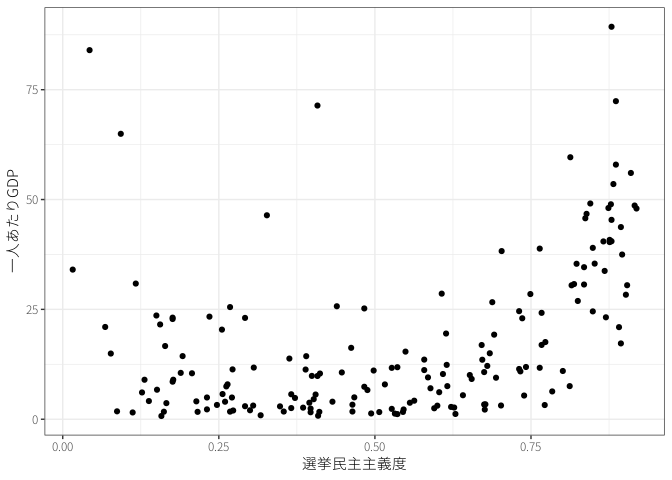
\includegraphics{war_and_diplomacy_files/figure-pdf/unnamed-chunk-2-1.png}

}

\caption{日米の国力比較(1900-45年)}

\end{figure}

\begin{itemize}
\tightlist
\item
  いずれアメリカと対決\(\leadsto\)国力が相対的に高いうちに攻撃してしまおうという動機?
\item
  現時点では戦争を回避できても、弱くなった将来において妥協を迫られるかもしれない。
\end{itemize}

圧倒的国力差にもかかわらず開戦するという、一見すると不合理な行動でも合理的に理解することはできる。

\hypertarget{ux5206ux5272ux4e0dux53efux80fdux6027}{%
\subsection{分割不可能性}\label{ux5206ux5272ux4e0dux53efux80fdux6027}}

交渉で戦争を回避できるための前提条件=財を分割できる。

\(\leadsto\)財が分割できない (indivisible)
場合=どちらか一方だけが全てを占有する (all or nothing)
場合\(\leadsto\)交渉の余地なし

\begin{itemize}
\tightlist
\item
  宗教上、神聖な土地
\item
  (ナショナリズムに深く根ざした)領域
\item
  イデオロギー、政治体制(の根本的な部分)
\end{itemize}

戦争の費用が十分に大きくない\(\leadsto\)交渉で解決不可能

\begin{itemize}
\tightlist
\item
  共同管理や補償によって分割可能にすることはできるかも?
\end{itemize}

\hypertarget{ux30a8ux30ebux30b5ux30ecux30e0}{%
\subsubsection{エルサレム}\label{ux30a8ux30ebux30b5ux30ecux30e0}}

エルサレム:キリスト教、ユダヤ教、イスラム教にとっての聖地

\begin{figure}[htpb]

{\centering \includegraphics[width=0.5\textwidth,height=\textheight]{war_and_diplomacy_files/mediabag/Westernwall2.jpg}

}

\caption{\href{https://commons.wikimedia.org/wiki/File:Westernwall2.jpg}{エルサレムの嘆きの壁と岩のドーム}}

\end{figure}

\begin{itemize}
\tightlist
\item
  1967年の\textbf{第3次中東戦争}(六日戦争)\(\leadsto\)イスラエルは東エルサレムを併合
\item
  1980年のエルサレム基本法:``The complete and united Jerusalem is the
  capital of Israel.''
\end{itemize}

\(\leadsto\)パレスチナも東エルサレムを首都としている\(\leadsto\)パレスチナ独立の大きな阻害要因

\hypertarget{ux30eaux30b9ux30afux614bux5ea6ux697dux89b3ux4e3bux7fa9}{%
\subsubsection{リスク態度・楽観主義}\label{ux30eaux30b9ux30afux614bux5ea6ux697dux89b3ux4e3bux7fa9}}

\textbf{リスク態度} (risk
attitude):不確実に得られるものに対して確実に得られるものを評価する態度\footnote{行動経済学の分野では利益を得る場合はリスク回避的、損失を受ける場合はリスク受容的になるというプロスペクト理論が知られている\citep{kahneman2013}。}

\begin{itemize}
\tightlist
\item
  譲歩をして確実に領土を得る(失う)or戦争でもしかすると領土を得られるかもしれないが失うかもしれない
\item
  \textbf{リスク受容的} (risk acceptant)
  な国家\(\leadsto\)交渉による確実な結果<戦争による不確実な結果\(\leadsto\)強硬姿勢
\item
  \textbf{楽観主義的} (optimistic)
  な国家\(\leadsto\)自国の勝利確率を過大に評価\(\leadsto\)強硬姿勢
\end{itemize}

\hypertarget{ux5b89ux5168ux4fddux969cux653fux7b56}{%
\section{安全保障政策}\label{ux5b89ux5168ux4fddux969cux653fux7b56}}

戦争=利害対立+外交の失敗

\(\leadsto\)安全保障政策=これらの要因を解消すること

\begin{itemize}
\tightlist
\item
  現状変更の意図:利害対立=現状変更勢力が戦争から得られる利益>平和から得られる利益。
\item
  情報の非対称性:現状維持勢力の抑止の決意を現状変更勢力が誤認
\item
  コミットメント問題:一方が相手の約束の信じることができない
\item
  分割不可能性:争っている財が分割不可能
\item
  リスク態度、楽観主義:戦争から得られる利益の過大評価
\end{itemize}

\(\leadsto\)特に最初の3つへの対処を考える。\footnote{分割不可能性やリスク態度、楽観主義は政策決定者の主観的要素であり、他者が変更することは難しい。}

\hypertarget{ux6226ux4e89ux306eux671fux9593ux7d42ux7d50}{%
\subsection{戦争の期間・終結}\label{ux6226ux4e89ux306eux671fux9593ux7d42ux7d50}}

戦争が外交の失敗\(\leadsto\)和平は外交の成功=外交の阻害要因がなくなれば成功するはず

\begin{itemize}
\tightlist
\item
  戦闘\(\leadsto\)能力や被害、決意が伝達\(\leadsto\)情報の非対称性の解消
\item
  戦闘\(\leadsto\)国力を低下\(\leadsto\)パワーシフト(によるコミットメント問題)の解消
\end{itemize}

データを用いた計量分析の結果\citep{weisiger2016}

\begin{figure}[htpb]

{\centering 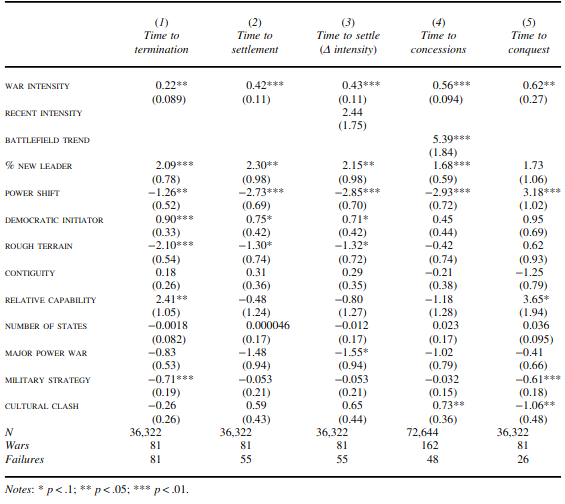
\includegraphics{figures/weisinger.png}

}

\caption{Battlefield deaths and war termination}

\end{figure}

\begin{itemize}
\tightlist
\item
  戦闘による情報の伝達は戦争の終結確率を高める。
\item
  国力を低下させることはより困難であるため大きなパワーシフトは戦争の終結確率は低くなる。
\end{itemize}


  \bibliography{references.bib}


\end{document}
